\section{组合图}
\label{sec:composite-plots}

前面介绍的绘图命令五花八门,但无论是plot、plot1或是plot2,同一个窗口内绘制的
所有波形总是共用同一个X轴。实际绘图时,经常需要在一张图中绘制多个不同X轴的图,
即组合图。

SAC提供了绘制组合图的功能,这其中牵涉到一些新的概念,其中之一是~\verb+frame+~。
一般而言,在执行绘图命令时会首先对整个窗口进行擦除。比如,先执行plot命令,窗口中
会显示出相应的波形,然后执行plot1命令,首先会将窗口中的已有图像全部擦除,再绘制
相应波形。

在frame中,每次执行绘图命令时,不会擦除窗口中的已有图像,从而实现了将多个命令的
绘图效果同时显示在一个窗口中。使用~\nameref{cmd:beginframe}~打开frame时,首先会
擦除整个窗口,进入``组合图模式'';当组合图绘制完成时,需要使用~\nameref{cmd:endframe}~
命令关闭frame。

除了frame之外,在绘制组合图时还需要了解与窗口有关的几个概念,如图
~\ref{fig:window-viewspace-viewport}:
\begin{itemize}
\item window:图形窗口。对于xwindows图形设备,window如图~\ref{fig:plot}~所示,
    其默认长宽比为11.0/8.5=1.294;对于sgf图形设备,可以认为window的大小即为A4纸张的大小。
\item viewspace:window内可以用于绘图的部分;
\item viewport:执行单个绘图命令时,图像的显示区域;
\end{itemize}

\begin{figure}[H]
\centering
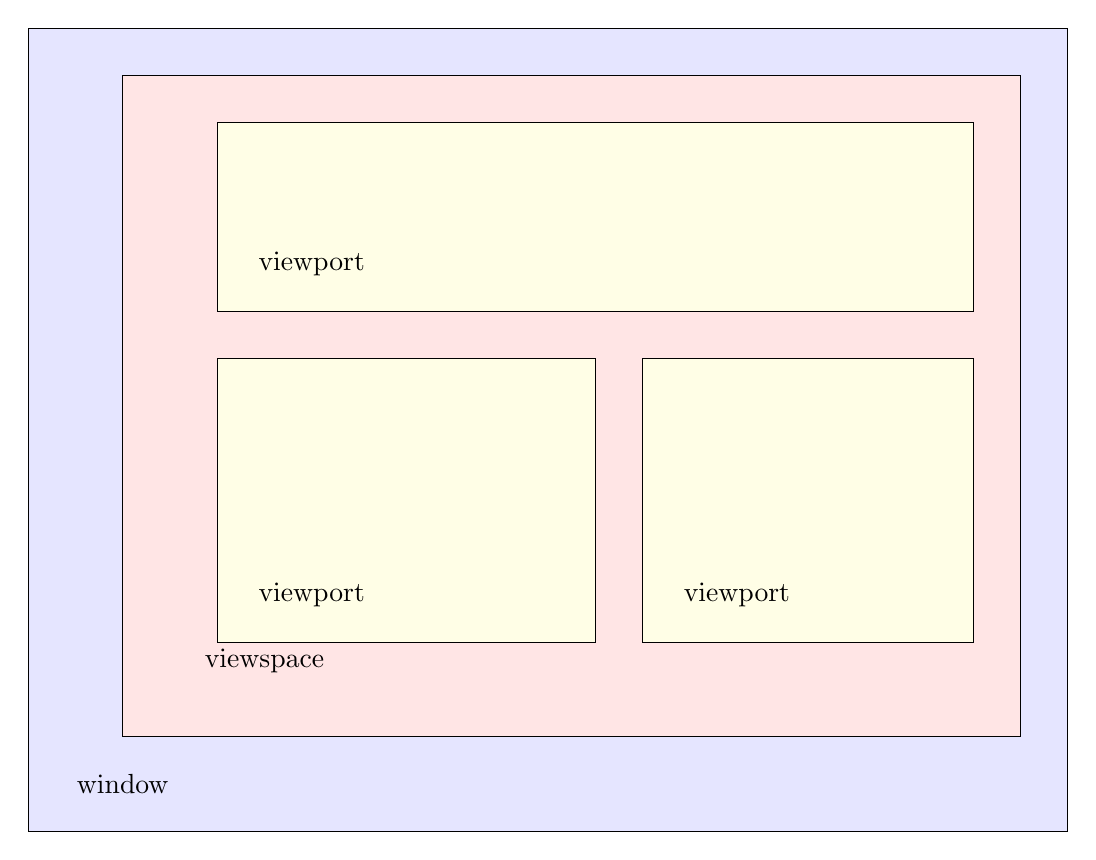
\begin{tikzpicture}[scale=1.2]
    \draw[fill=blue!10] (0,0) rectangle (11.0,8.5);
    \draw[fill=red!10] (1.0,1.0) rectangle (10.5,8);
    \draw[fill=yellow!10] (2,5.5) rectangle (10,7.5);
    \draw[fill=yellow!10] (2,2.0) rectangle (6,5.0);
    \draw[fill=yellow!10] (6.5,2.0) rectangle (10,5.0);
    \draw (1,0.5) node {window};
    \draw (2.5,1.8) node {viewspace};
    \draw (3.0,6) node {viewport};
    \draw (3.0,2.5) node {viewport};
    \draw (7.5,2.5) node {viewport};
\end{tikzpicture}
\caption{window、viewspace和viewport}
\label{fig:window-viewspace-viewport}
\end{figure}

图~\ref{fig:window-viewspace-viewport}~中给出了window、viewspace、viewport的相关
关系。可以使用~\nameref{cmd:window}~命令设定窗口相对于整个屏幕的位置以及X、Y方向
的范围;\nameref{cmd:vspace}~用于设定整个绘图区的比例;\nameref{cmd:xvport}~和
~\nameref{cmd:yvport}~则分别定义了单个绘图命令所能使用的X、Y方向的范围。

一个典型的组合图的绘制如下所示:
\begin{SACCode}
SAC> fg seis                        // 生成数据
SAC> beginframe                     // 打开frame,开始绘制组合图
SAC> xvport 0.1 0.9                 // 设定第一个绘图命令的viewport
SAC> yvport 0.7 0.9                 
SAC> title 'Seismic Trace'          // 设定标题
SAC> fileid off                     // 不显示文件id
SAC> qdp off                        
SAC> p                              
SAC> fft wmean                      // FFT
SAC> xvport .1 .45                  // 设定第二个绘图命令的viewport
SAC> yvport .15 .55
SAC> title 'Amplitude Response (linlog)'
SAC> ylim 1e-5 1                    // Y轴范围
SAC> psp am linlog                  // 绘制振幅谱(linlog)
SAC> xvport .55 .9                  // 设定第三个绘图命令的viewport
SAC> title 'Amplitude Response (loglog)'
SAC> xlim 1 60
SAC> psp am loglog                  // 绘制振幅谱(loglog)
SAC> endframe                       // 关闭frame
\end{SACCode}

\begin{figure}[H]
\centering
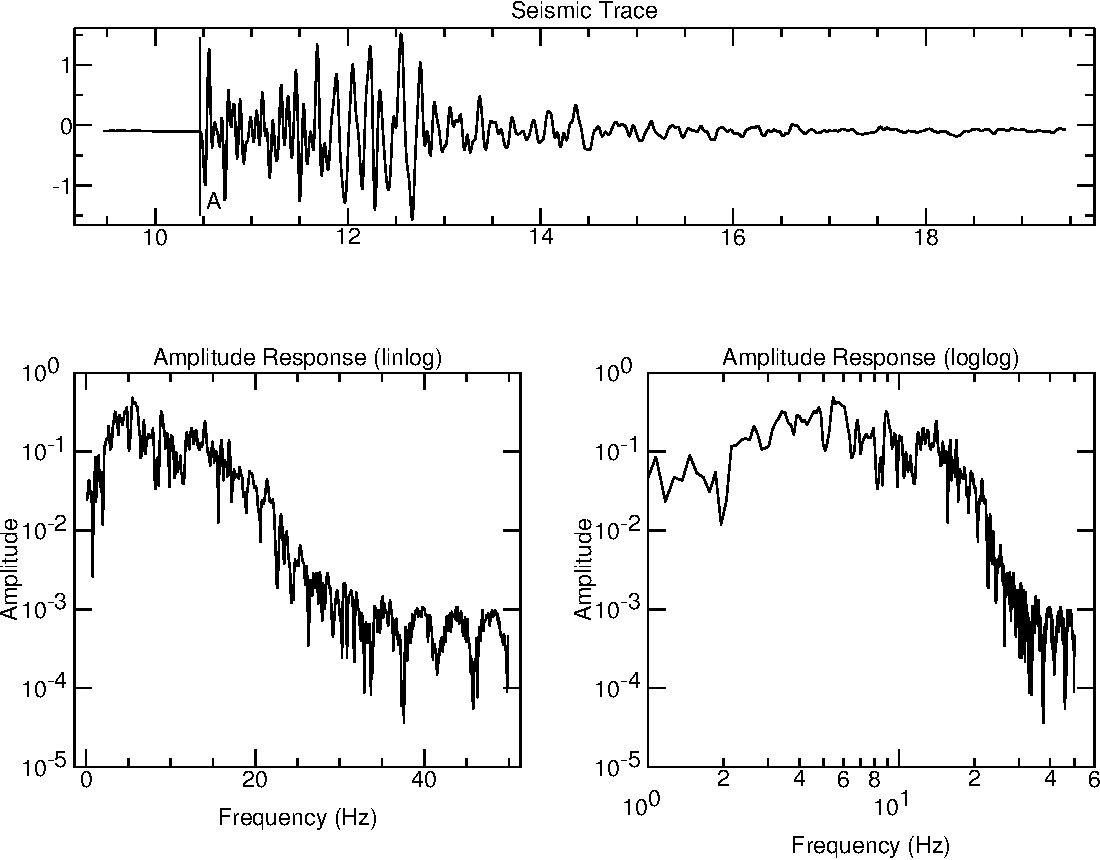
\includegraphics[width=0.9\textwidth]{composite-plot}
\caption{绘制组合图}
\label{fig:composite-plot}
\end{figure}
